\section{Results}
This part of the chapter provides the results of the experiment related to the two established hypotheses as well as insights gained from demographical information. Like with Experiment 1, data visualisation is provided by SPSS due to the large data file sizes. A significance level of 0.05 was used for all statistical tests. 

\subsection{Relative Effectiveness}
The first of the null hypotheses to be tested is effectiveness in terms of relative effectiveness. 

\subsubsection{Minimum Time Needed to Defeat Distractors}
As mentioned in Section~\ref{sec:ex2postprocessing}, in order to find a reasonable time period to discard unintentional resets in, it is first necessary to look at the minimum time needed to defeat any distractor. This can be seen in Figure~\ref{fig:minDistractorDefeatTime} where the minimum time is \textasciitilde18.23 seconds.

\begin{figure}[tbph]
    \centering
    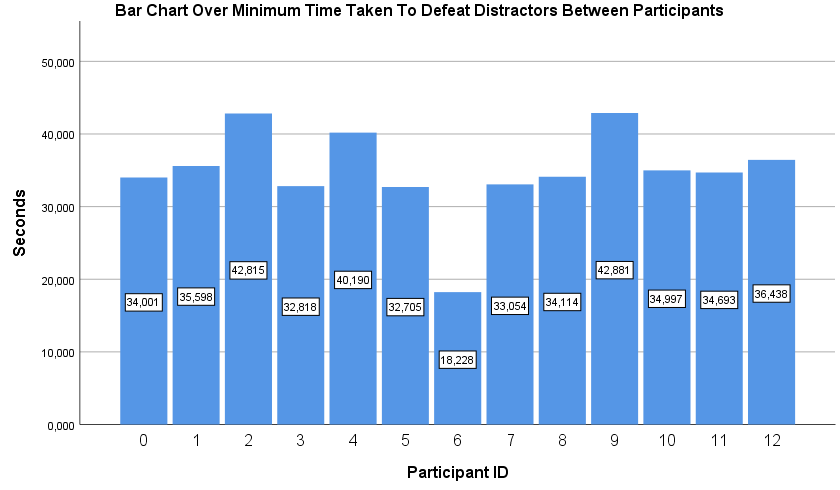
\includegraphics[width=0.75\textwidth]{figures/graphs/MinDistractorDefeatTime.png}
    \caption[Minimum Time Needed To Defeat Distractors Between Participants]{This bar chart shows the minimum time needed for each participant do defeat any distractor in Ensemble Retriever.}
    \label{fig:minDistractorDefeatTime}
\end{figure}

\subsubsection{Time and Walking Speed Normalisation}
Two variables that potentially could have some effect on the the reset counts between conditions is the time spent on walking and the walking speed of participants. It is thus necessary to first look at the mean movement speed and mean time spent on walking between the conditions before further analysis can take place. A boxplot on the time spent walking for participants between the two conditions can be seen in Figure~\ref{fig:TimeSpentWalkingBetweenConditions}. A boxplot on the mean metres per second that participants walked at between conditions can be seen in Figure~\ref{fig:ex2mps}.

\begin{figure}[tbph]
    \centering
    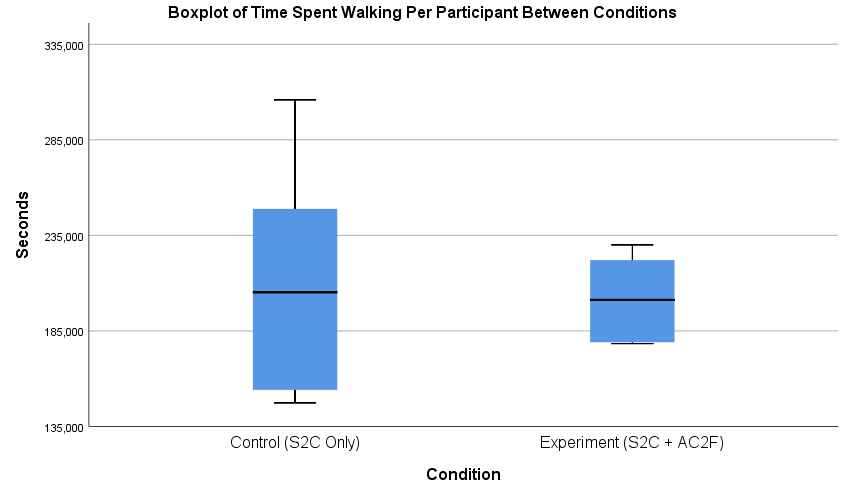
\includegraphics[width=0.75\textwidth]{figures/graphs/TimeSpentWalkingBetweenConditionsBoxPlot.png}
    \caption[Boxplot of Time Spent Walking Between Conditions in Experiment 2]{This boxplot shows the time that participants spent on walking between the two conditions.}
    \label{fig:TimeSpentWalkingBetweenConditions}
\end{figure}

\begin{figure}[tbph]
    \centering
    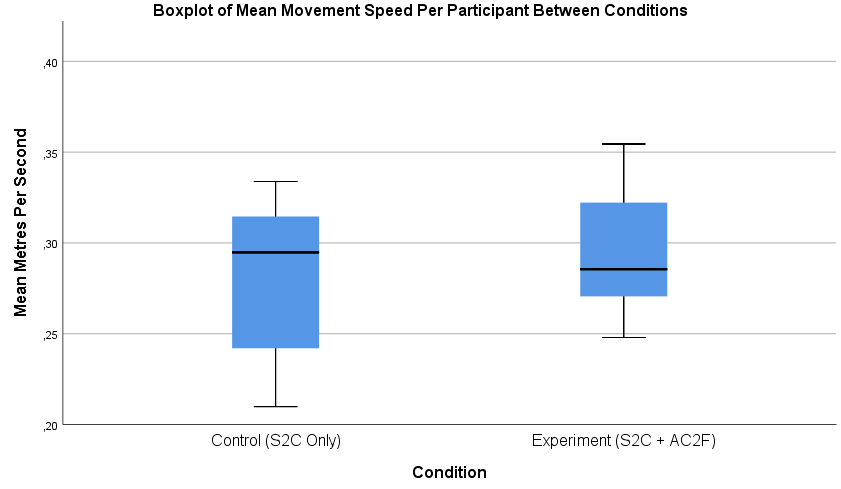
\includegraphics[width=0.75\textwidth]{figures/graphs/mpsBoxplot.png}
    \caption[Boxplot of Mean Walking Speed Between Conditions in Experiment 2]{This boxplot shows the mean walking speeds of participants between conditions.}
    \label{fig:ex2mps}
\end{figure}

A Shapiro-Wilk test was employed to check the normal distribution of these two variables. For the time spent walking, the test provided $p = 0.195$ for S2C Only and $p = 0.490$ for S2C+AC2F. Both conditions are as such normally distributed and a independent samples t-test was employed to look for statistically significant differences. The independent samples t-test yielded $t = 0.262, p = 0.798$ which means there is no statistical significance in terms of time spent walking. For clarity's sake, the mean walking time for S2C Only was 209.2 seconds and 202.0 seconds for S2C+AC2F. 

In terms of the mean walking speed, the Shapiro-Wilk test provided $p = 0.472$ for S2C Only and $p = 0.847$ for S2C+AC2F, meaning that the data is normally distributed. As such, an independent samples t-test was employed to look for statistically significant differences. 

   * T-test: t = -0.633, p = 0.540 
   * There is no statistical significance here either
   * Mean walking speed for S2C Only = 0.278 metres per second
   * Mean walking speed for S2C+AC2F = 0.294 metres per second
 
Since there is no statistically significant difference between the two conditions in terms of time spent walking or walking speed, further analysis will focus on the mean number of legitimate resets per participant. If there would have been a significant difference, a time or speed normalised variable would have needed to be calculated for comparisons. 

\subsubsection{Mean Number of Resets for Participants Between Conditions}
* Figure~\ref{fig:ex2resetMeans}.
\begin{figure}[tbph]
    \centering
    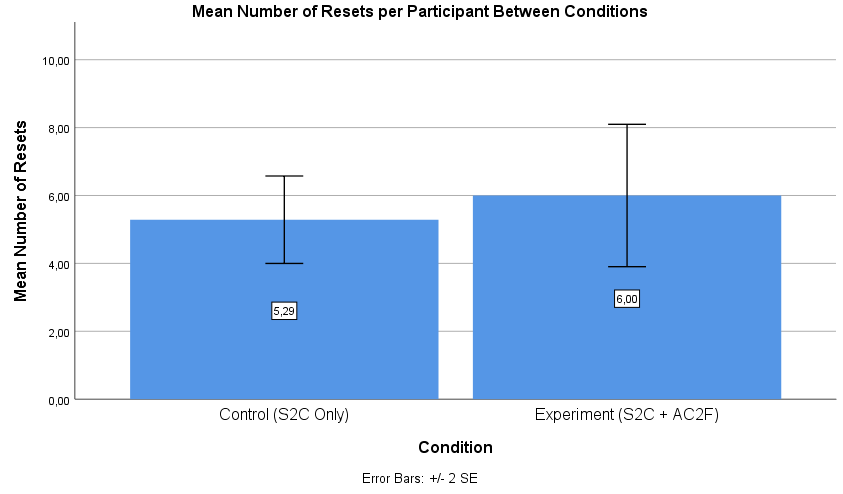
\includegraphics[width=0.75\textwidth]{figures/graphs/ResetMeans.png}
    \caption[Mean Number of Resets Between Conditions]{This bar chart shows the mean number of resets that participants experienced between conditions.}
    \label{fig:ex2resetMeans}
\end{figure}

\subsubsection{Hypothesis Testing}

\subsection{Alignment Time Effectiveness}

\subsection{Demographical Insights}

\subsubsection{Qualitative Feedback}